\documentclass{article}

\usepackage{float}
\usepackage[final]{graphicx}
\usepackage{subcaption}
\usepackage{multirow}
\usepackage{multicol}
\usepackage{blindtext}
\usepackage{hyperref}
\hypersetup{
    colorlinks=true,
    linkcolor=blue,
    filecolor=magenta,      
    urlcolor=blue,
    pdftitle={Overleaf Example},
    pdfpagemode=FullScreen,
    }

\title{\textbf{Machine Learning for detection of crop diseases}}
\author{Giovanni Belval}
\date{}

\begin{document}
\maketitle
\newpage

\begin{multicols}{2}
[
\section{Introduction}
]

The last few years , the world population has been growing faster and faster. This high rate of growth implies bigger and bigger ressources in order to feed humans. However , recent studies have shown that the crop yields only improve from 1.3$\%$ each years , instead of the $2.4\%$ required [1]. Moreover ,  crops are continuously threatened by various diseases. it is estimated that between 20\% and 40\% or yearly crops are lost each year due to diseases and insect pests , costing a global loss of \$200 billions and \$70 billions respectively [2]. In order to strop this trend , we could try to use more chemical products , but this is probably not the best solution. Increasing the amount of chemicals product will ultimately lead to more pollution of the soil , greater risk or humain health due to crops contaminations and finally , bacteria and insect will develop higher resistance , forcing us to use stronger and stronger chemical products.
in order to solve these problems , one can think about using Machine learning methods to detect and forecast crops diseases.\\
In this paper , I will try to develop some machine learning algorithms in order to detect crops diseases (mainly on tomatoes , potatoes and peppers) using the \textbf{PlantVillage} dataset  available on Kaggle [3].

\end{multicols}

\begin{multicols}{2}
[
\section{Data Exploration}
]

The \textbf{PlantVillage} Dataset gives us three categories of crop , \textbf{potatoes} ,  \textbf{tomatoes} (mainly) and  \textbf{peppers}. Our dataset contains pictures of tomatoes infected with \textbf{9} diseases/insects , potatoes with \textbf{2} , and peppers with only one disease , these information are listed in \textbf{Figure 1}. The entire Dataset is about $20000$. these images are already cleaned , so we don't have to do clean them ourselves.

\end{multicols}

\begin{figure}[H]
\centerline{\begin{tabular}{|c|c|c|c|}
\hline
\multirow{10}{*}{\textbf{Diseases}} & \textbf{Tomatoes}                      & \textbf{Potatoes} & \textbf{Peppers} \\ \cline{2-4} 
                                    & Target spot                            & Early blight      & Bacterial spot   \\ \cline{2-4} 
                                    & Mosaic virus                           & Late blight       &                  \\ \cline{2-4} 
                                    & YellowLeaf curl virus                  &                   &                  \\ \cline{2-4} 
                                    & Bacterial spot                         &                   &                  \\ \cline{2-4} 
                                    & Early blight                           &                   &                  \\ \cline{2-4} 
                                    & Spider mites  &                   &                  \\ \cline{2-4} 
                                    & Late blight                            &                   &                  \\ \cline{2-4} 
                                    & Leaf Mold                              &                   &                  \\ \cline{2-4} 
                                    & Septoria leaf spot                     &                   &                  \\ \hline
\end{tabular}}
\caption{Diseases per crops available in the dataset}
\end{figure}

\begin{multicols}{2}

having given an eye to the dataset , I found the dataset too "perfect" , images were always well delimited , oriented north etc. I was worried that a model trained on this dataset wouldn't be robust enough on real exemple (if I use my model on the real field , thus without clinical adjustments) so I made some data augmentation. Data added were randomly rotated , zoomed , or contrasted.
Some images of the initial dataset can be visualize in the \textbf{Figure 2} bellow. 

\end{multicols}

\begin{figure}[H]
\centering
\subfloat[potato with early blight]{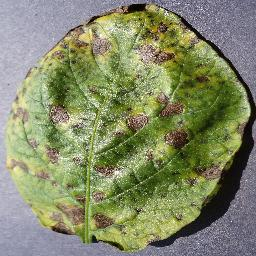
\includegraphics[width = 2in]{img/p_early}}
\subfloat[potato with late blight]{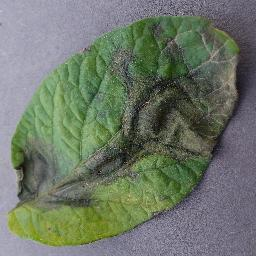
\includegraphics[width = 2in]{img/p_late}}\\
\subfloat[tomato leaf with bacterial spot]{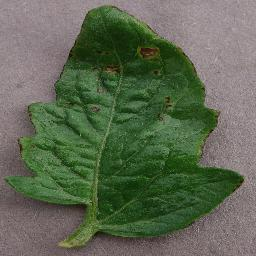
\includegraphics[width = 2in]{img/t_bspot}}
\subfloat[pepper leaf with bacterial spot]{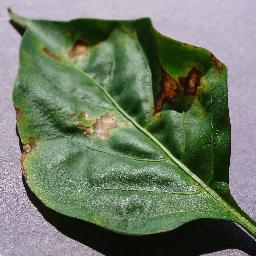
\includegraphics[width = 2in]{img/pe_bspot}} 
\caption{Random images from PlanVillage dataset}
\label{some examples}
\end{figure}

\newpage
\begin{multicols}{2}
[
\section{Model creation}
]

I created three different models , one for each type of crop. at the end , I also tried to create a model that can predict any categories from any crops. All the model and the code are available on \textbf{Github} [4]. The conception of the models are similar and not very hard. the main idea was to use convolutional layers  followed by Maxpooling Layer and finally connect it to fully connected layers.

\end{multicols}

\begin{figure}[H]

\centerline{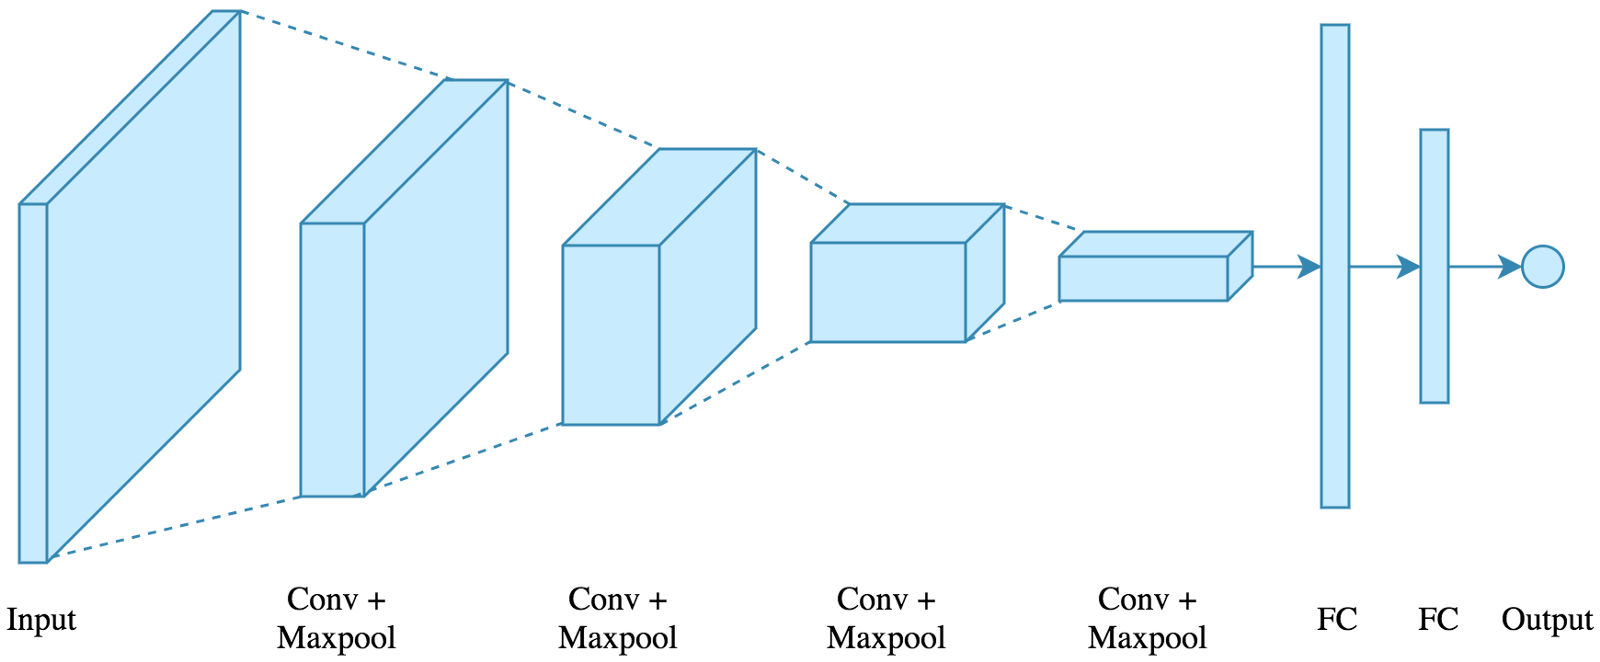
\includegraphics[scale = 0.25]{img/arch}}
\caption{Blue print of the models architecture }
\end{figure}

\begin{multicols}{2}
[
\section{Results}
]
The results are really promising , each model achieve a great performance on the test set as you can see in the \textbf{Figure 4}. there is no real differences between the final accuracy of each model (around 91\%).

\end{multicols}

\begin{figure}[H]
\centering
\begin{tabular}{|c|c|}
\hline
\textbf{Models}         & \textbf{Accuracy} \\ \hline
potatoes model & 0.92     \\ \hline
peppers model  & 0.99     \\ \hline
tomatoes model & 0.92     \\ \hline
global model   & 0.91     \\ \hline
\end{tabular}
\caption{Accuracies on the test sets}
\end{figure}

\begin{multicols}{2}
in y opinion , these results could be far better , especially for the global model. the main issus is that I used a very simple model containing only CNN layers and FC layers. One can add Batch Normalization layers and adding more layers in general. you can take a look at each model's structure on the report files available on my \textbf{Github} [4].
\end{multicols}

\begin{figure}[H]
\centerline{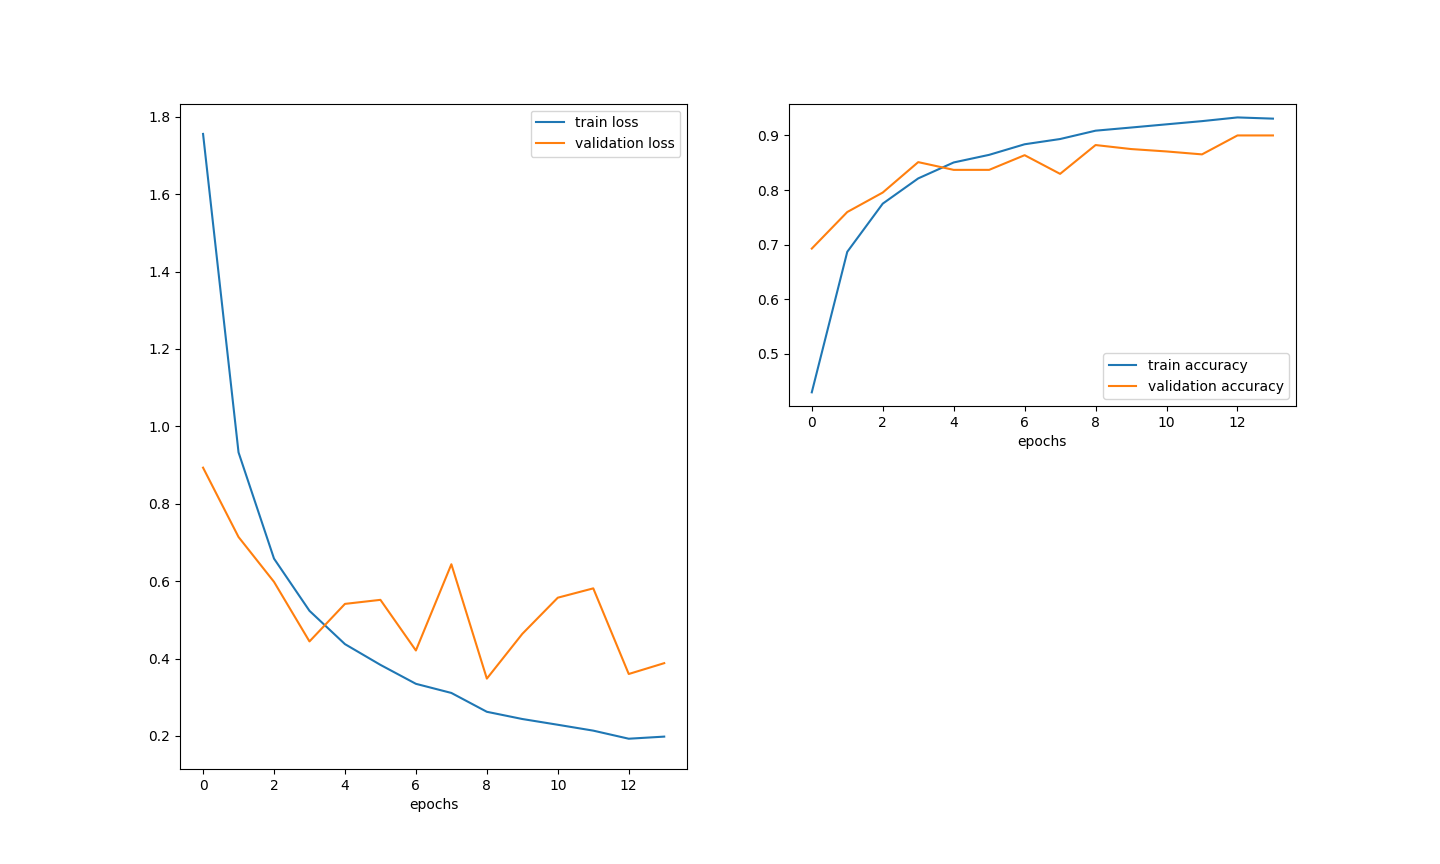
\includegraphics[scale=0.4]{img/global_results}}
\caption{Global model's loss and accuracy curves}
\end{figure}

\section{references}
1.  Roser, M. Future population growth. In Our World in Data; University of Oxford: Oxford, UK, 2013.\\
2. \href{https://www.agrivi.com/blog/yield-losses-due-to-pests}{https://www.agrivi.com/blog/yield-losses-due-to-pests} \\
3. \href{https://www.kaggle.com/datasets/emmarex/plantdisease}{https://www.kaggle.com/datasets/emmarex/plantdisease}\\
4.  \href{}{Github}

\end{document}